\documentclass[../resumosRCOM.tex]{subfiles}
\begin{document} 
\subsection{Introduction}
The medium access control (MAC) sublayer and the logical link control (LLC) sublayer together make up the data link layer.
\newline
\newline
The LLC sublayer provides multiplexing mechanisms that make it possible for several network protocols to coexist within a multipoint network and to be transported over the same network medium. It can also provide flow control and automatic repeat request (ARQ) error management mechanisms.
The LLC sublayer acts as an interface between the media access control (MAC) sublayer and the network layer.
\newline
\newline
When sending data to another device on the network, the MAC block encapsulates higher-level frames into frames appropriate for the transmission medium, adds a frame check sequence to identify transmission errors, and then forwards the data to the physical layer as soon as the appropriate channel access method permits it. Controlling when data is sent and when to wait is necessary to avoid congestion and collisions. Additionally, the MAC is also responsible for compensating for congestion and collisions by initiating retransmission if a jam signal is detected, and/or negotiating a slower transmission rate if necessary.
\newline
\subsection{Multiple Access Links}
\begin{itemize}
    \item \textbf {Point to Point} (single wire):
    \begin{itemize}
        \item PPP for dial-up access;
        \item Point-to-point link between Ethernet switch and host;
    \end{itemize}
    \item \textbf {Broadcast} (shared medium, wired or wireless):
    \begin{itemize}
        \item old-fashioned cabled Ethernet;
        \item 802.11 wireless LAN;
    \end{itemize}
\end{itemize}
\subsubsection{Ideal Multiple Access Protocol}
Used to coordinate the stations to use a common broadcast and shared channel of rate R bit/s.
\begin{itemize}
    \item \textbf {one} station wants to transmit -> it uses the \textbf {R} bit/s;
    \item \textbf {m} stations want to transmit -> each station uses an average rate \textbf {R/m} bit/s
    \item \textbf {simple} and \textbf {decentralized} (no coordination, no synchronization of clocks). 
\end{itemize}
\subsubsection{MAC Model and Concepts}
\textbf {Independent Traffic:} The model consists of N independent stations, each with a program or user that generates frames for transmission. The expected number of frames generated in an interval of length g is d*g, where d is a constant.Once a frame has been generated, the station is blocked and does nothing until the frame has been successfully transmitted. To analyze the protocols it uses Poisson Models.
\newline
\textbf {Single Channel:} A single channel is available for all communication. All stations can transmit on it and all can receive from it
\newline
\textbf {Collision:} Happens if two frames are transmitted simultaneously by different stations. A collided frame must be transmitted again later
\newline
\textbf {Continuous Time:} frame can be transmitted at any time.
\newline
\textbf {Slotted Time:} frame can be transmitted only at the beginning of a time slot.
\newline
\textbf {Carrier Sense:} station can know if medium (channel) is busy before using it.
\newline
\textbf {No Carrier Sense:} station cannot sense channel before using it.
\newline
Poisson models
\subsection{MAC Protocols}
The MAC Protocols can be separated into Three Classes: Channel Partitioning, Random Access and Taking turns.
\subsection{Channel Partitioning}
Divide channel into smaller "pieces" (time slots,frequency).
\newline
The communication resource is partitioned in N channels that are assigned to stations is a quasi-static way. 
\newline
Poor efficiency on low loaded channels.
\newline The principle protocols are:
\begin{itemize}
        \item Time Division Multiplexing;
        \item Frequency Division Multiplexing.
\end{itemize}
\subsection{Random access protocols}
\begin{itemize}
        \item Each station tries to access the full communication resource in a random, uncoordinated manner -> collisions occur;
        \item Poor efficiency on highly loaded channels;
        \item When station has packet to send a packet,transmits at channel data rate \textbf{R} bit/s.
        \item Random Access MAC protocol defines:
        \begin{itemize}
        \item when to send data;
        \item how to detect collisions;
        \item how to recover from collisions.
\end{itemize}
\end{itemize}

\subsubsection{Pure ALOHA}
Aloha is a technique for coordinating the access of large numbers of intermittent transmitters in a single shared communication channel.
\newline
\begin{itemize}
\item In Aloha, whenever a station has data, it transmits it;
\item If more than one frames are transmitted, they collide and are lost. The Sender finds out whether the transmission was successful or experienced a collision by listening to the broadcast from the
destination station;
\item If ACK (signal that data has been received successfully) not received within timeout, then a station picks random backoff algorithm to re-transmit;
\item After the backoff time, the station re-transmits the frame.
\end{itemize}

\begin{figure}[H]
    \centering
    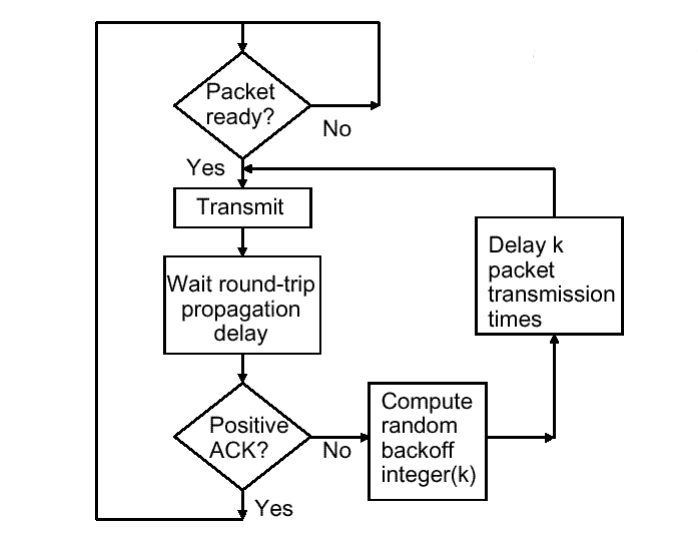
\includegraphics[scale=0.3]{Mac_1.png}
    \caption{Station behaviour}
\end{figure}

\subsubsection{Slotted ALOHA}
In the Slotted ALOHA, the time is divided into time slots and each slot corresponds to one frame.
\newline
A station is not permitted to send whenever the user types a line. Instead, it is required to wait for the beginning of the next slot and the stations transmit frames only at the beginning of a time slot.
\newline
This method causes a reduction on the collision probability.

\begin{figure}[H]
    \centering
    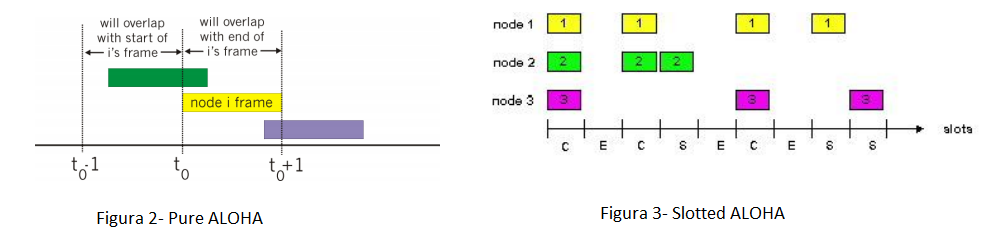
\includegraphics[scale=0.5]{Mac_2.png}
\end{figure}
\textbf{ALOHA Efficiency:}
\begin{figure}[H]
    \centering
    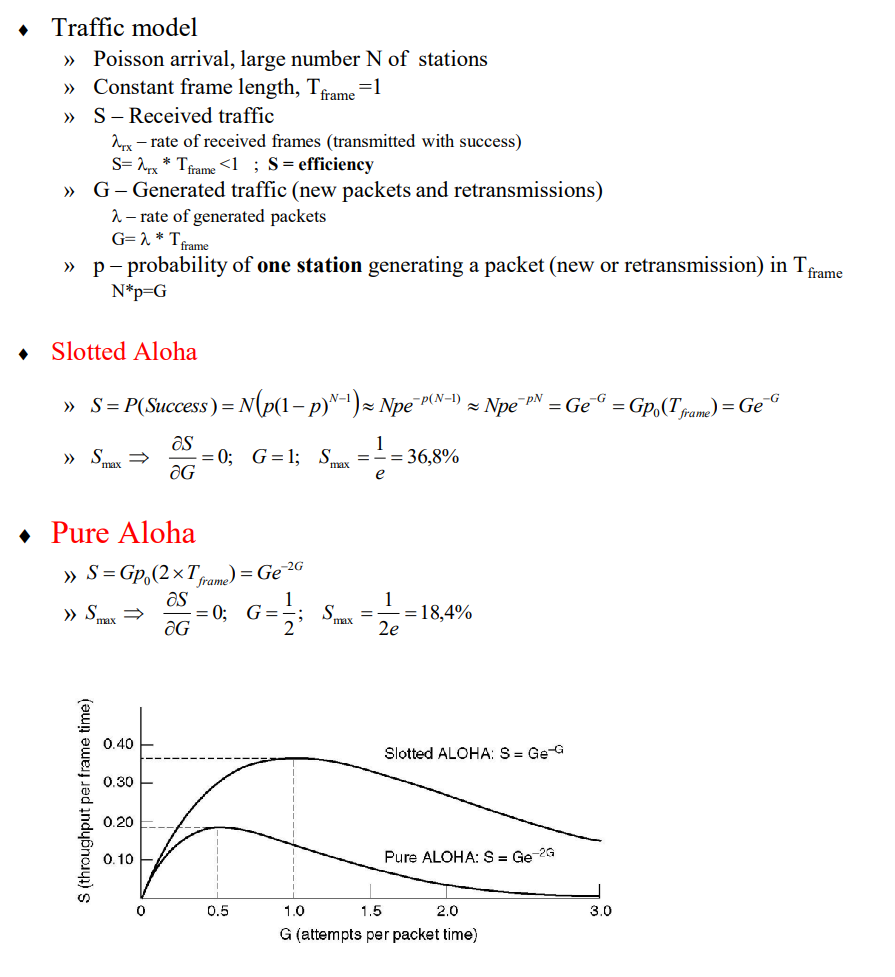
\includegraphics[scale=0.5]{Mac_3.png}
\end{figure}


\subsubsection{CSMA (Carrier Sense Multiple Access)}
Carrier-sense multiple access (CSMA) is a media access control (MAC) protocol in which a node verifies the absence of other traffic before transmitting on a shared transmission medium.
\newline
A transmitter attempts to determine whether another transmission is in progress before initiating a transmission using a carrier-sense mechanism. If a carrier is sensed, the node waits for the transmission in progress to end before initiating its own transmission.
\newline
\textbf{Persistency} - what to do after the medium is found busy
\newline
\newline
\textbf{CSMA collisions:}
\begin{itemize}
        \item Collisions can still occur due to a propagation delay or because stations may not hear other transmissions;
        \item When a collision happens the station waits random time and repeats algorithm;
        \item Collision vulnerability time = 2*Tprop;
        \item Collision probability = a = Tprop/Tframe;
\end{itemize}
\textbf{CSMA Variants:}
\begin{itemize}
        \item CSMA \textbf {1-persistent:} If the channel is idle (free), the stations sends its data. Otherwise, if the channel is busy, the station just waits until it becomes idle. Then the station transmits a frame.
        \item CSMA \textbf {Non-persistent:} If the channel is idle, the stations sends its data. Otherwise, if the channel is busy, the station waits a random time and repeats algorithm
        \item CSMA \textbf {p-persistent:} If the channel is idle, it transmits 
        with a probability p. With a probability $q = 1 - p$, it defers until the 
        next slot. If that slot is also idle, it either transmits or defers again, 
        ith probabilities p and q. This process is repeated until either the frame 
        has been transmitted or another station has begun transmitting. In the latter 
        case, the unlucky station acts as if there had been a collision. If the station
         initially senses that the channel is busy, it waits until the next slot and 
         applies the algorithm above.
\end{itemize}
\begin{figure}[H]
    \centering
    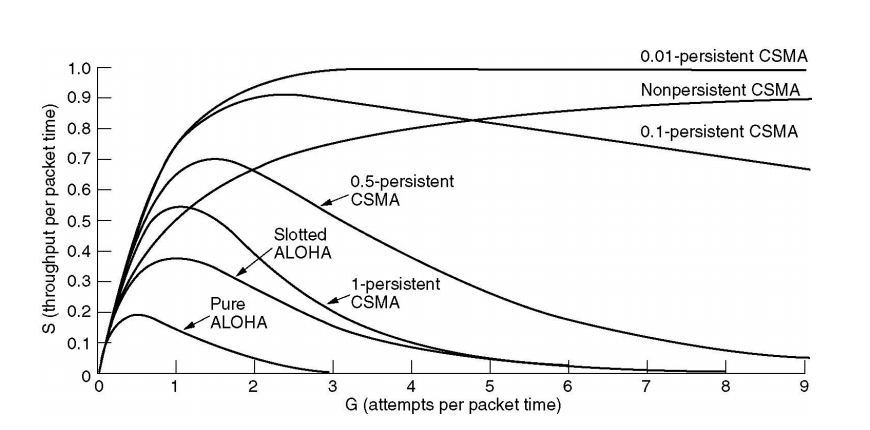
\includegraphics[scale=0.4]{Mac_4.png}
    \caption{Efficiencies}
\end{figure}
\subsubsection{CSMA with Collision Detection (CSMA/CD)}
CSMA/CD operates by detecting the occurrence of a collision. Once a collision is detected, CSMA/CD immediately terminates the transmission thus shortening the time required before a retry can be attempted. The last information can be re-transmitted.
\newline
CSMA/CD is used by Ethernet.
\newline
\begin{itemize}
    \item \textbf{Carrier Sense:} Station senses medium before transmitting. If free, station starts transmission. If busy, waits until its free and then transmits (= 1-persistent)
    \item \textbf{Collision Detection:} If collision is detected,the transmission is aborted and the re-transmission is delayed using a Binary Exponential Back-off algorithm.
    \item \textbf{Binary Exponential Back-off algorithm:}
    \begin{itemize}
        \item Time is modeled in time slots and each Tslot= 2*Tprop;
        \item After the i consecutive collision -> waits a random number of slots uniformly distributed in [0, 2i-1] and attemps to re-transmit.
    \end{itemize}
    \item \textbf{Doesn't use ACK}.
    \item To detected a collision,\textbf{Tframe>2*Tprop}.
\end{itemize}
\begin{figure}[H]
    \centering
    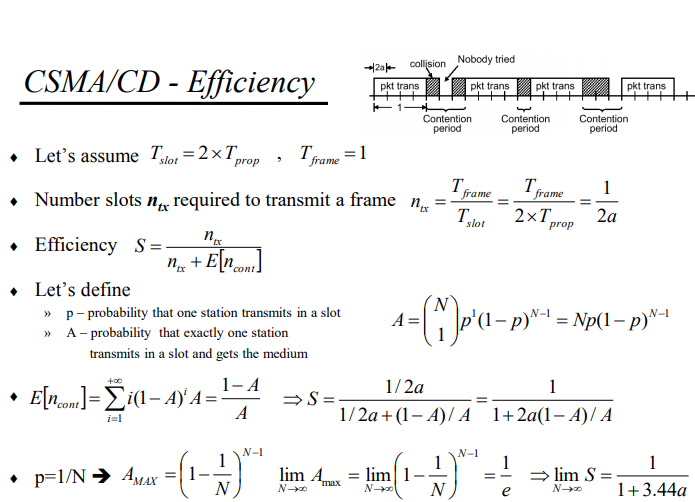
\includegraphics[scale=0.5]{Mac_5.png}
\end{figure}
\subsubsection{CSMA with Collision Avoidance (CSMA/CA)}
Carrier-sense multiple access with collision avoidance (CSMA/CA) is a network multiple access method in which carrier sensing is used, but nodes attempt to avoid collisions by beginning transmission only after the channel is sensed to be idle. When they do transmit, nodes transmit their packet data in its entirety.
\newline
It is an unreliable method
\begin{itemize}
    \item if medium free, transmits frame
    \item if medium busy:
    \begin{itemize}
        \item Random backoff interval is selected which will be decremented as long as the channel is sensed idle;
        \item Stopped when a transmission is detected on the channel;
        \item Re-activated when the channel is sensed idle again for more than a DIFS;
        \item The station transmits when the backoff time reaches 0.
    \end{itemize}
    \item To avoid channel capture, station waits random backoff time between two consecutive frame transmissions, even if the medium is sensed idle in the DIFS time.
    \item \textbf{It uses ACKs}.
\end{itemize}
\begin{figure}[H]
    \centering
    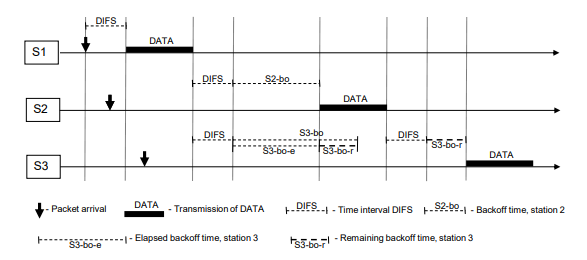
\includegraphics[scale=0.5]{Mac_6.png}
\end{figure}
\subsubsection{Taking-turns protocols}
Tightly coordinate shared access to avoid collisions.
\newline
Usage of the communication resource is disciplined by some turning mechanisms.
\begin{itemize}
    \item Each station has its own turn;
    \item Stations with more information to send, might have bigger turns;
    \item \textbf{Polling:}
    \begin{itemize}
        \item Controlled by a master station which invites slave stations to transmit in turn.
        \item \textbf{concerns}: polling overhead; latency; single point of failure (master).
    \end{itemize}
    \item \textbf{Token passing:}
    \begin{itemize}
        \item The stations will pass the control token from one station to next sequentially, warning which is able to transmit.
        \item \textbf{concerns}: token overhead; latency; single point of failure (token).
    \end{itemize}
\end{itemize}
\subsection{MAC}

The standard for wireless LANs is called IEEE 802.11, aka WiFi.
\newline
The most common type of wired LANs is called IEEE 803.2, aka Ethernet.
\begin{itemize}
    \item 48 bit address
    \item Unique for each adaptor
    \item Broadcast address FF-FF-FF-FF-FF-FF
\end{itemize}
\subsection{Ethernet}
\begin{itemize}
    \item Bus Topology :
    \subitem Popular in the mid 90s
    \subitem Stations in same collision domain
    \item Star Topology :
    \subitem Current Topology
    \subitem Active switch in center
    \subitem Each station runs individual Ethernet protocols
    \subitem Stations do not collide with each other
    \item \textbf{Full-Duplex}: The stations don't have to wait for each other and there is no collision. The CSMA/CD algorithm is not needed.
\end{itemize}
\subsection{Switch}
\begin{itemize}
    \item Link-layer device
    \item Forwards Ethernet frames
    \item Transparent to hosts
    \item Does not need to be configured
    \item Has forwarding table
\end{itemize}
\subsubsection{When the Switch receives a frame:}
\begin{itemize}
    \item Records link associated with sending host
    \item index forwarding tabel using MAC destination address
    \item if entry is found in table
    \subitem if destination is on segment from which frame arrived,
    \subsubitem drop the frame
    \subitem else
    \subsubitem forward the frame on interface indicated
    else flood (forward on all but the interface on which the frame arrived)
\end{itemize}
\subsection{Virtual LANs}
\begin{itemize}
    \item One bridge/switch simulates multiple LANs/broadcast domains
    \item One LAN may be extended to other bridges
\end{itemize}
\subsection{Previous Exams Questions:}
\begin{figure}[H]
    \centering
    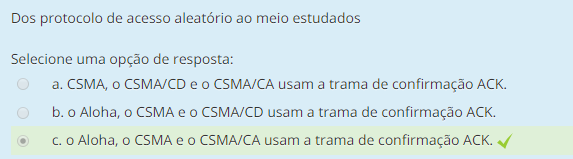
\includegraphics[scale=0.5]{Mac_7.png}
    \newline
    \newline
    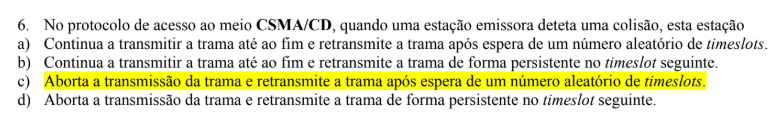
\includegraphics[scale=0.5]{Mac_8.png}
    \newline
    \newline
    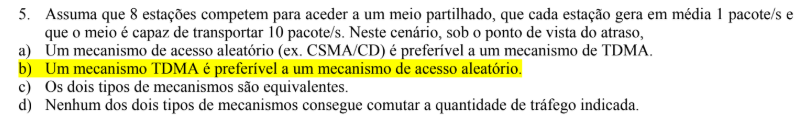
\includegraphics[scale=0.5]{Mac_9.png}
    \newline
    \newline
    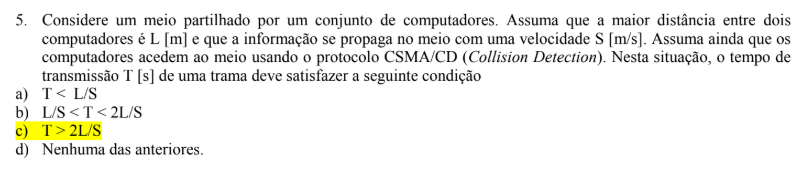
\includegraphics[scale=0.5]{Mac_10.png}
    \newline
    \newline
    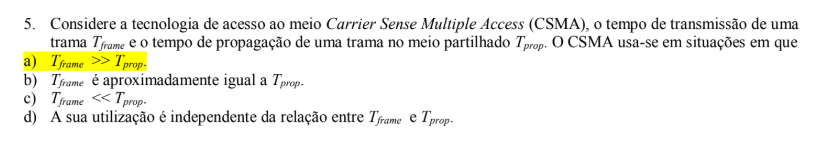
\includegraphics[scale=0.5]{Mac_11.png}
    \newline
    \newline
    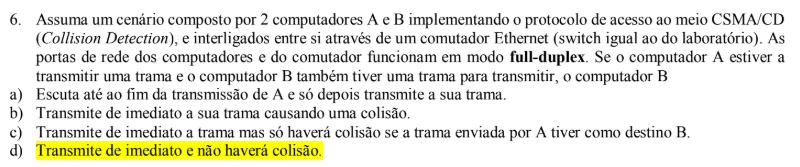
\includegraphics[scale=0.5]{Mac_12.png}
    \newline
    \newline
    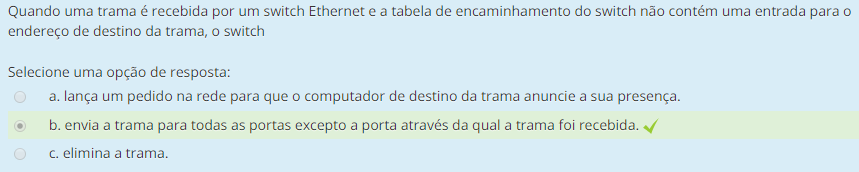
\includegraphics[scale=0.5]{Mac_13.png}
\end{figure}
\end{document}